%!TEX root = ../../Master.tex
When designing an interactive system it is important to think about the people using it. The people are a part of the interactive system and therefore it is important to make sure that the design fits the people. In~\cite{benyon2013designing} PACT analysis is presented as a framework for thinking about design situations. To help with the design being human centred, the designer needs to understand the four parts of the analysis: It is important to understand the different kind of people using the system, since they have different prerequisites for using a system. The activities that people want to undertake are equally important, as it says a lot about the way the system will be used. The designer needs to think about the context, the location and organisation, the system will be used in, which provide information about how the system should operate. Lastly the designer should consider the features of interactive technologies and how to incorporate them in the design.

\begin{figure}
  \centering
  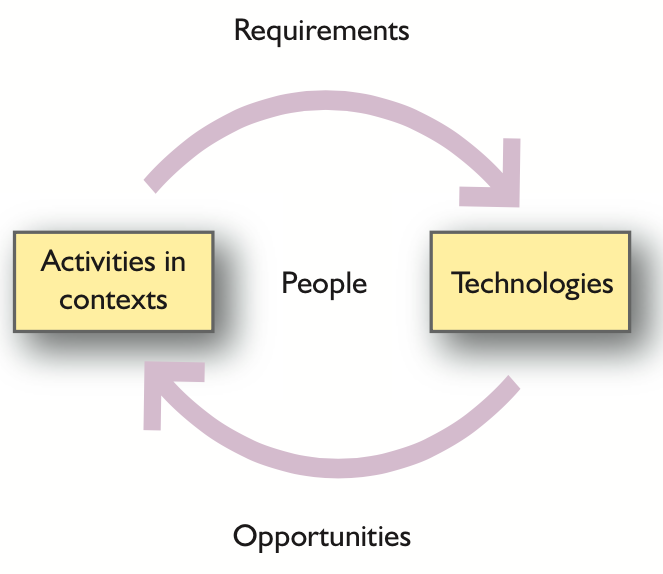
\includegraphics[width=0.5\linewidth]{pact-overview.png}
  \caption{The relationships between activities, contexts, people and technologies in PACT. From~\cite{benyon2013designing}}
  \label{fig:pact-overview}
\end{figure}

It is also important to understand the relationship between activities and technologies. \Cref{fig:pact-overview} shows how the activities people are doing will influence the requirements for technologies. This will create new technology that will change the activities people will be doing with the technology.

It is the variety of requirements that is found during the PACT analysis, that can make designing systems difficult. Therefore, an analysis of the four core elements of PACT will be conducted.


\subsection{People}
\label{sub:pact_people}

The system is used by people who go to bar-like environments, and are possibly intoxicated. At bar-like environments, music is central to the atmosphere, and a lot of people are interested in having their music tastes accommodated. Different people exhibit different behaviour in these social contexts, some may clique together when using a social system and some may be afraid of stigmas when using it. To use the system, a smartphone is required, and some people may be unable or afraid \chnote{uddyb hvorfor} to use their smartphone.

\subsection{Activities}
\label{sub:pact_activities}

Usage of the system requires the user to interact with their smartphone or similar device. Firstly the user must install the application on their device. The installation process should not take a long time, or else the user might forget about the application. When the user is checked-in, the current playlist of the venue will be displayed. The transition from the check-in to the playlist screen should occur in less than 100 milliseconds as to not frustrate the user. From the playlist screen the user can vote on a track. Finding which track to vote for should not be a complex action, as this is an expected frequently done action.

\paragraph{New or improved activities}
The system introduces a possibility of requesting a track to be played at the venue, without having to ask the administrator. This eases work load on administrator, which might be busy serving beverages to a customer. It also eases the process of requesting a track by not having to get up if sitting and splitting from one's group or partner, which may lead to a more time spend together. The system might change the behavior of the users and serve as topic of discussion, possibly an icebreaker. These changes in activities should be considered when designing the system.

\subsection{Context}
\label{sub:pact_context}

This system can be used at places where many people wants to listen to music, but does not have an efficient method \chnote{påstand, uddyb} of determining which tracks to listen to.

A dark environment with a lot of noise is common in bars/pubs. As people are often dancing in this environment, active use of smartphones is not recommended\chnote{why}. Also, usage of smartphones in these kind of environments often cause anti-social behaviour. \chnote{kilde ville være super nice :)}

\subsection{Technologies}
\label{sub:pact_technologies}

The system runs on a host computer with an audio system connected and a business license for Spotify. \chnote{meget specific?} This host computer is located at the installation site.

For users to operate this system a smartphone with internet connection and adequate battery life is required. \chnote{ved vi alle de ting? hvis det skal ikke skal være i retrospekt}
When designing the system, different smartphones and their characteristics have to be considered.

\subsection{Summary}
\label{sec:pact_summary}

The people using the system are possibly intoxicated, and most likely in the context of meeting and talking to other people. It is often considered rude and anti-social to neglect the people you are with, by using a smartphone. In order to minimise this behaviour, the system must be \textit{quick}\footnote{Frequent and determined users might access the system often with a already known task for the system, making them capable of communicating a request of system very quickly, the system should sought to not be the limiting factor in this process.} and \textit{easy to navigate and use}, by providing a small and effective set of functionalities. 
Power consumption on the mobile devices is of concern, as smartphones usually drain their batteries quickly when in active use. Therefore a requirement of the system is to \textit{minimize power consumption}, by not doing extensive computing on the clients side.


The PACT analysis provides us with the following requirements
\begin{itemize}
  \item Should be quicker than the user
  \item Easy to use and navigate - Few but effective functionalities
  \item No unnecessary computations on the client
\end{itemize}